\section{Results}
With the materials and methods that have been described, we have executed a MapReduce job on the CTIT cluster. This job has counted the tweets that have been sent about a game on every day from December 2010 until November 2015. These tweet counts have been processed and their results have been made visible using highcharts, one of which can be seen below. We chose to use highcharts, because they contain some handy functions such as zooming in on a particular time period. The full results for all of the games in the top 20 can be found on the website that we have created. \footnote{http://wiefferink.me/GameTweets}.

\begin{figure}[!ht]
	\centering
	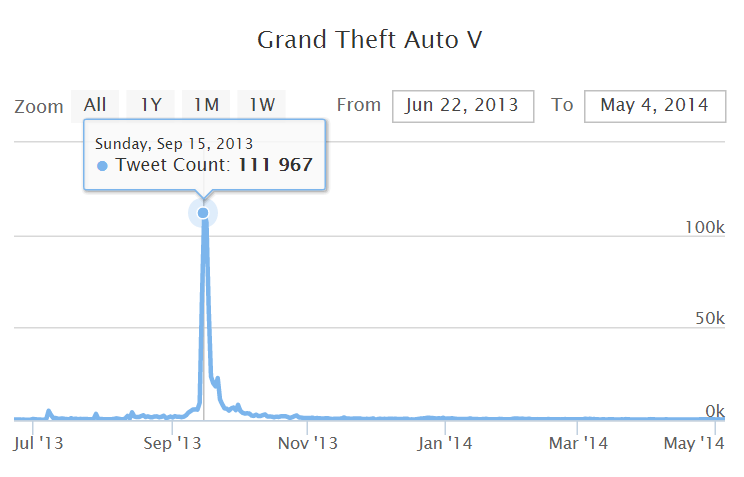
\includegraphics[width=0.4\textwidth]{highchart-gta3}
	\caption{Highchart for the game Grand Theft Auto V (zoomed in around the release date).}
	\label{highchartgta}
\end{figure}
\FloatBarrier

This image \ref{highchartgta} represents the amount of tweets that were sent daily about the game Grand Theft Auto V.  The release date for the game was September 17th, 2013.

The main result of this research was to check for a correlation between the amount of tweets that were sent about a certain game, and its position in the sales charts. For the purpose of checking for such a correlation, we decided to take the Twitter results and the sales charts, and create a list that contains both for all of the games. This list has been included in this report as \ref{resultNumbers}.